% Created 2025-05-21 Wed 10:07
% Intended LaTeX compiler: pdflatex
\documentclass[a4paper,12pt]{article}
\usepackage[utf8]{inputenc}
\usepackage[T1]{fontenc}
\usepackage{amsmath}
\usepackage{amssymb}
\usepackage{capt-of}
\usepackage{hyperref}
\usepackage{amsthm}
\usepackage{amssymb}
\usepackage{mathtools}
%\documentclass[12pt]{article}
\usepackage{geometry}

\usepackage{amsmath}
\usepackage{amssymb,amsfonts,textcomp}
\usepackage[T1]{fontenc}
\usepackage[utf8]{inputenc}
\usepackage{times} % Times New Roman font
\usepackage{setspace}
\usepackage[pdftex]{graphicx}

\usepackage{hyperref}

% Set line spacing to 1.5
\setstretch{1.5}

\geometry{a4paper, portrait, margin=0.7in, nohead}

\usepackage{titlesec}
\titleformat{\section}[block]{\normalfont\large\bfseries}{\thesection}{1em}{}
\titleformat{\subsection}[block]{\normalfont\large\bfseries}{\thesubsection}{1em}{}

\makeatletter

\newcommand{\student}[1]{\author{#1}}

\newcommand{\group}[1]{\def\@group{#1}}

\newcommand{\prof}[1]{\def\@prof{#1}}
\newcommand{\profdep}[1]{\def\@profdep{#1}}

\newcommand{\labno}[1]{\def\@labno{#1}}

\newcommand{\labtopic}[1]{\title{#1}}

\group{FAF--233}
\prof{Fistic Cristofor}
\profdep{sea, fcim utm}
\labno{5}

%% ox-latex features:
%   !announce-start, !guess-pollyglossia, !guess-babel, !guess-inputenc,
%   engraved-code, caption, maths, image, !announce-end.

% Setup for code blocks [1/2]

\usepackage{fvextra}

\fvset{%
  commandchars=\\\{\},
  highlightcolor=white!95!black!80!blue,
  breaklines=true,
  breaksymbol=\color{white!60!black}\tiny\ensuremath{\hookrightarrow}}

% Make line numbers smaller and grey.
\renewcommand\theFancyVerbLine{\footnotesize\color{black!40!white}\arabic{FancyVerbLine}}

\usepackage{xcolor}

% In case engrave-faces-latex-gen-preamble has not been run.
\providecolor{EfD}{HTML}{f7f7f7}
\providecolor{EFD}{HTML}{28292e}

% Define a Code environment to prettily wrap the fontified code.
\usepackage[breakable,xparse]{tcolorbox}
\providecommand{\codefont}{\footnotesize}
\DeclareTColorBox[]{Code}{o}%
{colback=EfD!98!EFD, colframe=EfD!95!EFD,
  fontupper=\setlength{\fboxsep}{0pt}\codefont,
  colupper=EFD,
  IfNoValueTF={#1}%
  {boxsep=2pt, arc=2.5pt, outer arc=2.5pt,
    boxrule=0.5pt, left=2pt}%
  {boxsep=2.5pt, arc=0pt, outer arc=0pt,
    boxrule=0pt, leftrule=1.5pt, left=0.5pt},
  right=2pt, top=1pt, bottom=0.5pt,
  breakable}

% Support listings with captions
\usepackage{float}
\floatstyle{plain}
\newfloat{listing}{htbp}{lst}
\newcommand{\listingsname}{Listing}
\floatname{listing}{\listingsname}
\newcommand{\listoflistingsname}{List of Listings}
\providecommand{\listoflistings}{\listof{listing}{\listoflistingsname}}


% Setup for code blocks [2/2]: syntax highlighting colors

\newcommand\efstrut{\vrule height 2.1ex depth 0.8ex width 0pt}
\definecolor{EFD}{HTML}{000000}
\definecolor{EfD}{HTML}{ffffff}
\newcommand{\EFD}[1]{\textcolor{EFD}{#1}} % default
\definecolor{EFh}{HTML}{7f7f7f}
\newcommand{\EFh}[1]{\textcolor{EFh}{#1}} % shadow
\definecolor{EFsc}{HTML}{228b22}
\newcommand{\EFsc}[1]{\textcolor{EFsc}{\textbf{#1}}} % success
\definecolor{EFw}{HTML}{ff8e00}
\newcommand{\EFw}[1]{\textcolor{EFw}{\textbf{#1}}} % warning
\definecolor{EFe}{HTML}{ff0000}
\newcommand{\EFe}[1]{\textcolor{EFe}{\textbf{#1}}} % error
\definecolor{EFc}{HTML}{b22222}
\newcommand{\EFc}[1]{\textcolor{EFc}{#1}} % font-lock-comment-face
\definecolor{EFcd}{HTML}{b22222}
\newcommand{\EFcd}[1]{\textcolor{EFcd}{#1}} % font-lock-comment-delimiter-face
\definecolor{EFs}{HTML}{8b2252}
\newcommand{\EFs}[1]{\textcolor{EFs}{#1}} % font-lock-string-face
\definecolor{EFd}{HTML}{8b2252}
\newcommand{\EFd}[1]{\textcolor{EFd}{#1}} % font-lock-doc-face
\definecolor{EFm}{HTML}{008b8b}
\newcommand{\EFm}[1]{\textcolor{EFm}{#1}} % font-lock-doc-markup-face
\definecolor{EFk}{HTML}{9370db}
\newcommand{\EFk}[1]{\textcolor{EFk}{#1}} % font-lock-keyword-face
\definecolor{EFb}{HTML}{483d8b}
\newcommand{\EFb}[1]{\textcolor{EFb}{#1}} % font-lock-builtin-face
\definecolor{EFf}{HTML}{0000ff}
\newcommand{\EFf}[1]{\textcolor{EFf}{#1}} % font-lock-function-name-face
\definecolor{EFv}{HTML}{a0522d}
\newcommand{\EFv}[1]{\textcolor{EFv}{#1}} % font-lock-variable-name-face
\definecolor{EFt}{HTML}{228b22}
\newcommand{\EFt}[1]{\textcolor{EFt}{#1}} % font-lock-type-face
\definecolor{EFo}{HTML}{008b8b}
\newcommand{\EFo}[1]{\textcolor{EFo}{#1}} % font-lock-constant-face
\definecolor{EFwr}{HTML}{ff0000}
\newcommand{\EFwr}[1]{\textcolor{EFwr}{\textbf{#1}}} % font-lock-warning-face
\newcommand{\EFnc}[1]{#1} % font-lock-negation-char-face
\definecolor{EFpp}{HTML}{483d8b}
\newcommand{\EFpp}[1]{\textcolor{EFpp}{#1}} % font-lock-preprocessor-face
\newcommand{\EFrc}[1]{\textbf{#1}} % font-lock-regexp-grouping-construct
\newcommand{\EFrb}[1]{\textbf{#1}} % font-lock-regexp-grouping-backslash
\newcommand{\EFob}[1]{#1} % org-block
\definecolor{EFhn}{HTML}{008b8b}
\newcommand{\EFhn}[1]{\textcolor{EFhn}{#1}} % highlight-numbers-number
\definecolor{EFhq}{HTML}{9370db}
\newcommand{\EFhq}[1]{\textcolor{EFhq}{#1}} % highlight-quoted-quote
\definecolor{EFhs}{HTML}{008b8b}
\newcommand{\EFhs}[1]{\textcolor{EFhs}{#1}} % highlight-quoted-symbol
\definecolor{EFrda}{HTML}{707183}
\newcommand{\EFrda}[1]{\textcolor{EFrda}{#1}} % rainbow-delimiters-depth-1-face
\definecolor{EFrdb}{HTML}{7388d6}
\newcommand{\EFrdb}[1]{\textcolor{EFrdb}{#1}} % rainbow-delimiters-depth-2-face
\definecolor{EFrdc}{HTML}{909183}
\newcommand{\EFrdc}[1]{\textcolor{EFrdc}{#1}} % rainbow-delimiters-depth-3-face
\definecolor{EFrdd}{HTML}{709870}
\newcommand{\EFrdd}[1]{\textcolor{EFrdd}{#1}} % rainbow-delimiters-depth-4-face
\definecolor{EFrde}{HTML}{907373}
\newcommand{\EFrde}[1]{\textcolor{EFrde}{#1}} % rainbow-delimiters-depth-5-face
\definecolor{EFrdf}{HTML}{6276ba}
\newcommand{\EFrdf}[1]{\textcolor{EFrdf}{#1}} % rainbow-delimiters-depth-6-face
\definecolor{EFrdg}{HTML}{858580}
\newcommand{\EFrdg}[1]{\textcolor{EFrdg}{#1}} % rainbow-delimiters-depth-7-face
\definecolor{EFrdh}{HTML}{80a880}
\newcommand{\EFrdh}[1]{\textcolor{EFrdh}{#1}} % rainbow-delimiters-depth-8-face
\definecolor{EFrdi}{HTML}{887070}
\newcommand{\EFrdi}[1]{\textcolor{EFrdi}{#1}} % rainbow-delimiters-depth-9-face


\usepackage{capt-of}

\usepackage{amsmath}
\usepackage{amssymb}

\usepackage{graphicx}

%% end ox-latex features


\author{Andrei Chicu}
\date{\today}
\title{Study and empirical analysis of greedy algorithms: Prim's Algorithm and Kruskal's Algorithm}
\hypersetup{
 pdfauthor={Andrei Chicu},
 pdftitle={Study and empirical analysis of greedy algorithms: Prim's Algorithm and Kruskal's Algorithm},
 pdfkeywords={},
 pdfsubject={},
 pdfcreator={Emacs 30.1 (Org mode 9.8-pre)},
 pdflang={English}}
\begin{document}

\makeatletter
\begin{titlepage}
\centering


\includegraphics[height=2cm]{utm_logo.png}

\bfseries
\textsc{Ministry of Education and Research of Republic of Moldova} \\
\textsc{Technical University of Moldova} \\
\textsc{Faculty of Computers, Informatics and Microelectronics} \\
\textsc{Department of Software and Automation Engineering} \\
\mdseries

\vfill

\textsc{\Large Analysis of Algorithms} \\
\textsc{\large Laboratory work \#\@labno}\\[0.5cm]

\vspace{12pt}
\newcommand{\HRule}{\rule{\linewidth}{0.5mm}}
\HRule \\[0.2cm]
{ \LARGE \bfseries \@title }\\[0.4cm]
\HRule
\vfill

\begin{minipage}[t]{0.4\textwidth}
\begin{flushleft} \large
\emph{Author:} \\
\@author\\                        
std. gr. \@group
\end{flushleft}
\end{minipage}
~
\begin{minipage}[t]{0.4\textwidth}
\raggedleft \large
\emph{Verified:} \\
\@prof \\
Department of \textsc{\@profdep}
\end{minipage}\\[3cm]
\vfill

Chișinău, 2025
\end{titlepage}
\makeatother
\setcounter{page}{2}
\section{Analysis of Algorithms}
\label{sec:orgf3bae42}
github url: \url{https://github.com/andyp1xe1/aa_labs/tree/main/lab5}
\subsection{Objective}
\label{sec:org536cbc5}
The objective of this laboratory work is to implement and analyze two fundamental greedy algorithms for finding minimum spanning trees: Prim's Algorithm and Kruskal's Algorithm. The analysis aims to compare their performance across various graph types and sizes to understand their efficiency characteristics, time complexity behavior, and practical applications in different graph scenarios.
\subsection{Tasks}
\label{sec:org3f954ef}
1 Study the greedy algorithm design technique.
2 To implement in a programming language algorithms Prim and Kruskal. 
3 Empirical analyses of the Kruskal and Prim
4 Increase the number of nodes in graph and analyze how this influences the algorithms. Make a graphical presentation of the data obtained
5 To make a report.
\subsection{Theoretical Notes}
\label{sec:org01eb287}

This lab explores greedy algorithms for finding minimum spanning trees in graphs. Below, we discuss the theoretical background and algorithms implemented.
\subsubsection{Minimum Spanning Tree}
\label{sec:org7d8a195}
A minimum spanning tree (MST) of a connected, undirected, weighted graph is a tree that spans all vertices with the minimum possible total edge weight. MSTs have numerous practical applications in network design, circuit wiring, cluster analysis, and approximation algorithms for NP-hard problems like the Traveling Salesman Problem. The key property of an MST is that it provides the lowest-cost way to connect all vertices in a graph, ensuring network connectivity while minimizing resource usage (e.g., cable length, construction costs). Both Prim's and Kruskal's algorithms exploit the greedy property that locally optimal choices at each step lead to a globally optimal spanning tree. For any connected graph, the MST is unique if all edge weights are distinct; otherwise, multiple MSTs may exist with the same total weight.
\subsubsection{Types of Graphs}
\label{sec:org969d2c6}
In this laboratory, we analyze the algorithms on the following types of graphs:
\begin{enumerate}
\item Complete Graph
\label{sec:org1703710}
Every vertex is connected to every other vertex, resulting in |V|(|V|-1)/2 edges in an undirected graph.
\item Dense Graph
\label{sec:orgc7e2485}
Has approximately 80\% of the maximum possible edges.
\item Sparse Graph
\label{sec:org8e13bea}
Contains relatively few edges, approximately 2|V| edges.
\item Connected Graph
\label{sec:orgd8732b9}
There exists a path between any pair of vertices.
\item Grid Graph
\label{sec:org28d2315}
Vertices arranged in a grid-like structure with connections primarily to adjacent nodes.
\end{enumerate}
\subsubsection{Greedy Algorithms}
\label{sec:orgd3e3eac}
A greedy algorithm is an approach for solving a problem by selecting the best option available at the moment. It doesn't worry whether the current best result will bring the overall optimal result. The algorithm never reverses the earlier decision even if the choice is wrong. It works in a top-down approach. This algorithm may not produce the best result for all the problems. It's because it always goes for the local best choice to produce the global best result.
\subsubsection{Prim's Algorithm}
\label{sec:orgc0f5427}
Prim's algorithm builds the MST one vertex at a time, starting from an arbitrary root vertex and at each step adding the lowest-weight edge that connects the tree to a vertex not yet in the tree. The algorithm works as follows:

\begin{enumerate}
\item Initialize a tree with a single vertex, chosen arbitrarily from the graph
\item Grow the tree by one edge at a time: of the edges that connect the tree to vertices not yet in the tree, find the minimum-weight edge and add it to the tree
\item Repeat step 2 until all vertices are in the tree
\end{enumerate}

Prim's algorithm has time complexity O(E log V) when implemented with a binary heap, where E is the number of edges and V is the number of vertices.
\subsubsection{Kruskal's Algorithm}
\label{sec:org46b01e9}
Kruskal's algorithm builds the MST by adding edges in order of increasing weight, skipping edges that would create a cycle. The algorithm works as follows:

\begin{enumerate}
\item Sort all the edges in non-decreasing order of their weight
\item Initialize an empty forest (set of trees) where each vertex is a separate tree
\item For each edge in the sorted list:
\begin{itemize}
\item If adding this edge does not create a cycle (vertices are in different trees), add it to the forest and merge the trees
\item Otherwise, discard this edge
\end{itemize}
\item Continue until the forest becomes a tree (or all edges have been processed)
\end{enumerate}

Kruskal's algorithm has time complexity O(E log E) or equivalently O(E log V), dominated by the sorting step, where E is the number of edges and V is the number of vertices.
\subsection{Comparison Metric}
\label{sec:org83ab280}
For this empirical analysis, we measure the following metrics:

\begin{enumerate}
\item \textbf{\textbf{Execution Time}}: The primary metric is the actual execution time in seconds for each algorithm across different graph types and sizes. This provides an empirical measure of the algorithm's efficiency.

\item \textbf{\textbf{Number of Edges in MST}}: This will always be V-1 for a connected graph with V vertices, serving as a validation check.

\item \textbf{\textbf{Total Weight of MST}}: The sum of weights of all edges in the resulting MST. Both algorithms should produce the same total weight for the same input graph.
\end{enumerate}

The algorithms are evaluated on various graph types with sizes ranging from 100 to 2500/10,000 vertices to observe how they scale with input size.

\begin{Code}
\begin{Verbatim}
\color{EFD}\EFv{sizes} \textcolor[HTML]{000000}{=} [10, 50, 60, 70, 80, 90, 100, 150, 200, 300]
\EFv{mid\_sizes} \textcolor[HTML]{000000}{=} [100, 200, 300, 500, 700, 1000]
\end{Verbatim}
\end{Code}

For each graph type and size, algorithms were executed with 5 repetitions to account for system variability and provide statistical robustness. This approach allows us to:

\begin{itemize}
\item Calculate mean execution times for more reliable performance comparison
\item Determine standard deviation to assess result consistency and reliability
\item Identify potential outliers or anomalous behavior in specific test cases
\end{itemize}

The error bars in the plots represent the standard deviation across these repetitions, providing a visual indication of measurement variability.
\subsection{Input Format}
\label{sec:org48b6592}
In this laboratory work, graphs are represented using adjacency lists implemented as nested Python dictionaries. Each vertex is a key in the outer dictionary, and its value is another dictionary mapping neighboring vertex IDs to edge weights.

For MST algorithms, we convert the directed graph representation to an undirected one by ensuring each edge appears in both directions with the same weight.

Example input graph structure:
\begin{Code}
\begin{Verbatim}
\color{EFD}\EFv{graph} \textcolor[HTML]{000000}{=} \{
    \EFs{'0'}: \{\EFs{'1'}: 5, \EFs{'2'}: 3\},
    \EFs{'1'}: \{\EFs{'0'}: 5, \EFs{'3'}: 2, \EFs{'4'}: 4\},
    \EFs{'2'}: \{\EFs{'0'}: 3\},
    \EFs{'3'}: \{\EFs{'1'}: 2\},
    \EFs{'4'}: \{\EFs{'1'}: 4, \EFs{'2'}: 1\}
\}
\end{Verbatim}
\end{Code}

In this representation:
\begin{itemize}
\item Vertices '0' and '1' are connected by an edge with weight 5
\item Vertices '0' and '2' are connected by an edge with weight 3
\item Vertices '1' and '3' are connected by an edge with weight 2
\item Vertices '1' and '4' are connected by an edge with weight 4
\item Vertices '4' and '2' are connected by an edge with weight 1
\end{itemize}

All graphs are generated with the functions provided in the uploaded code, with vertices labeled as strings from '0' to 'n-1' and edge weights ranging from 1 to 10.
\section{Implementation}
\label{sec:orgd9d1a1b}
\subsection{Prim's Algorithm}
\label{sec:org6dc86c1}
Prim's algorithm is implemented using a priority queue to efficiently find the minimum-weight edge at each step. We use a min-heap data structure from Python's heapq module.
\begin{listing}[htbp]
\begin{Code}
\begin{Verbatim}
\color{EFD}\EFk{def} \EFf{prims}(graph, start\textcolor[HTML]{000000}{=}\EFo{None}):
    \EFk{import} heapq

    \EFcd{\# }\EFc{Extract all vertices}
    \EFv{vertices} \textcolor[HTML]{000000}{=} \EFb{list}(graph.keys())

    \EFk{if} \EFk{not} vertices:
        \EFk{return} [], [], 0

    \EFcd{\# }\EFc{Use provided start vertex or default to first vertex}
    \EFk{if} start \EFk{is} \EFo{None} \EFk{or} start \EFk{not} \EFk{in} vertices:
        \EFv{start} \textcolor[HTML]{000000}{=} vertices[0]

    \EFcd{\# }\EFc{Initialize tracking structures}
    \EFv{visited} \textcolor[HTML]{000000}{=} \{start\}
    \EFv{tree\_edges} \textcolor[HTML]{000000}{=} []
    \EFv{explored\_edges} \textcolor[HTML]{000000}{=} []

    \EFcd{\# }\EFc{Priority queue to store edges (weight, from\_vertex, to\_vertex)}
    \EFv{edge\_queue} \textcolor[HTML]{000000}{=} []
    \EFk{for} neighbor, weight \EFk{in} graph[start].items():
        heapq.heappush(edge\_queue, (weight, start, neighbor))

    \EFk{while} edge\_queue \EFk{and} \EFb{len}(visited) \textcolor[HTML]{000000}{<} \EFb{len}(vertices):
        \EFv{weight}, \EFv{from\_vertex}, \EFv{to\_vertex} \textcolor[HTML]{000000}{=} heapq.heappop(edge\_queue)

        \EFcd{\# }\EFc{Record this exploration}
        explored\_edges.append((from\_vertex, to\_vertex, weight))

        \EFk{if} to\_vertex \EFk{in} visited:
            \EFk{continue}

        \EFcd{\# }\EFc{Add edge to minimum spanning tree}
        tree\_edges.append((from\_vertex, to\_vertex, weight))
        visited.add(to\_vertex)

        \EFcd{\# }\EFc{Add all edges from the new vertex to priority queue}
        \EFk{for} neighbor, edge\_weight \EFk{in} graph[to\_vertex].items():
            \EFk{if} neighbor \EFk{not} \EFk{in} visited:
                heapq.heappush(edge\_queue, (edge\_weight, to\_vertex, neighbor))

    \EFcd{\# }\EFc{Calculate total weight of MST}
    \EFv{mst\_weight} \textcolor[HTML]{000000}{=} \EFb{sum}(weight \EFk{for} \_, \_, weight \EFk{in} tree\_edges)

    \EFk{return} tree\_edges, explored\_edges, mst\_weight
\end{Verbatim}
\end{Code}
\caption{\label{lst:org5e22850}Implementation of Prim's Algorithm}
\end{listing}
\clearpage
\subsection{Kruskal's Algorithm}
\label{sec:orgee918c1}
Kruskal's algorithm is implemented using a disjoint-set data structure (Union-Find) to efficiently detect cycles. We sort edges by weight and add them to the MST if they don't create cycles.
\begin{listing}[htbp]
\begin{Code}
\begin{Verbatim}
\color{EFD}\EFk{def} \EFf{kruskal}(graph, start\textcolor[HTML]{000000}{=}\EFo{None}):
    \EFcd{\# }\EFc{Define disjoint-set data structure for cycle detection}
    \EFk{class} \EFt{DisjointSet}:
        \EFk{def} \EFf{\_\_init\_\_}(\EFk{self}, vertices):
            \EFk{self}.\EFv{parent} \textcolor[HTML]{000000}{=} \{v: v \EFk{for} v \EFk{in} vertices\}
            \EFk{self}.\EFv{rank} \textcolor[HTML]{000000}{=} \{v: 0 \EFk{for} v \EFk{in} vertices\}

        \EFk{def} \EFf{find}(\EFk{self}, vertex):
            \EFk{if} \EFk{self}.parent[vertex] \textcolor[HTML]{000000}{!=} vertex:
                \EFk{self}.\EFv{parent}[vertex] \textcolor[HTML]{000000}{=} \EFk{self}.find(\EFk{self}.parent[vertex])
            \EFk{return} \EFk{self}.parent[vertex]

        \EFk{def} \EFf{union}(\EFk{self}, vertex1, vertex2):
            \EFv{root1} \textcolor[HTML]{000000}{=} \EFk{self}.find(vertex1)
            \EFv{root2} \textcolor[HTML]{000000}{=} \EFk{self}.find(vertex2)

            \EFk{if} root1 \textcolor[HTML]{000000}{!=} root2:
                \EFk{if} \EFk{self}.rank[root1] \textcolor[HTML]{000000}{<} \EFk{self}.rank[root2]:
                    \EFk{self}.\EFv{parent}[root1] \textcolor[HTML]{000000}{=} root2
                \EFk{elif} \EFk{self}.rank[root1] \textcolor[HTML]{000000}{>} \EFk{self}.rank[root2]:
                    \EFk{self}.\EFv{parent}[root2] \textcolor[HTML]{000000}{=} root1
                \EFk{else}:
                    \EFk{self}.\EFv{parent}[root2] \textcolor[HTML]{000000}{=} root1
                    \EFk{self}.\EFv{rank}[root1] \textcolor[HTML]{000000}{+=} 1
                \EFk{return} \EFo{True}
            \EFk{return} \EFo{False}

    \EFcd{\# }\EFc{Extract all vertices}
    \EFv{vertices} \textcolor[HTML]{000000}{=} \EFb{list}(graph.keys())

    \EFk{if} \EFk{not} vertices:
        \EFk{return} [], [], 0

    \EFcd{\# }\EFc{Collect all edges}
    \EFv{edges} \textcolor[HTML]{000000}{=} []
    \EFk{for} vertex \EFk{in} vertices:
        \EFk{for} neighbor, weight \EFk{in} graph[vertex].items():
            \EFcd{\# }\EFc{Prevent duplicate edges by only adding if vertex < neighbor}
            \EFk{if} vertex \textcolor[HTML]{000000}{<} neighbor:
                edges.append((weight, vertex, neighbor))

    \EFcd{\# }\EFc{Sort edges by weight}
    edges.sort()

    \EFcd{\# }\EFc{Initialize DisjointSet}
    \EFv{ds} \textcolor[HTML]{000000}{=} DisjointSet(vertices)

    \EFcd{\# }\EFc{Track results}
    \EFv{tree\_edges} \textcolor[HTML]{000000}{=} []
    \EFv{explored\_edges} \textcolor[HTML]{000000}{=} []

    \EFcd{\# }\EFc{Process edges in ascending order of weight}
    \EFk{for} weight, vertex1, vertex2 \EFk{in} edges:
        \EFcd{\# }\EFc{Record this exploration}
        explored\_edges.append((vertex1, vertex2, weight))

        \EFk{if} ds.union(vertex1, vertex2):
            \EFcd{\# }\EFc{Edge is part of MST}
            tree\_edges.append((vertex1, vertex2, weight))

    \EFcd{\# }\EFc{Calculate total weight of MST}
    \EFv{mst\_weight} \textcolor[HTML]{000000}{=} \EFb{sum}(weight \EFk{for} \_, \_, weight \EFk{in} tree\_edges)

    \EFk{return} tree\_edges, explored\_edges, mst\_weight
\end{Verbatim}
\end{Code}
\caption{\label{lst:orgb8883f7}Implementation of Kruskal's Algorithm}
\end{listing}
\section{Results}
\label{sec:org82a1865}
\subsection{Complete Graph}
\label{sec:org082c07d}
\begin{center}
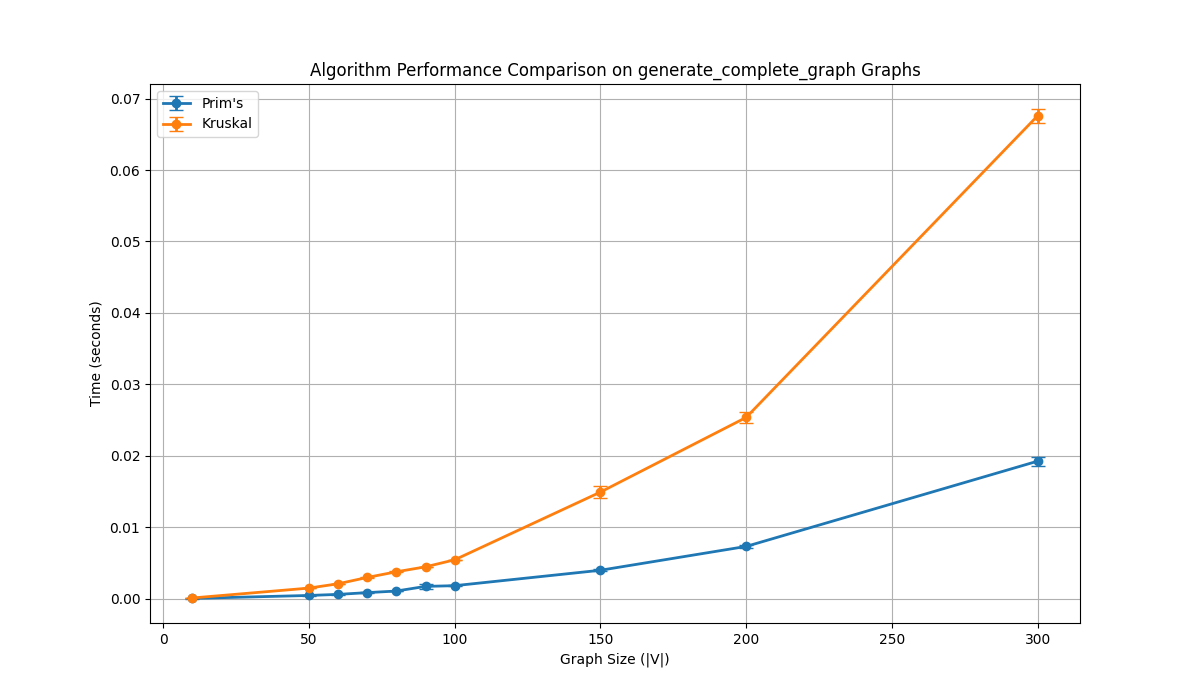
\includegraphics[width=.9\linewidth]{mst_complete.png}
\label{org3a279fe}
\end{center}

For complete graphs, the execution time for both algorithms shows a clear polynomial growth pattern as graph size increases. From the data presented in the figure, Kruskal's algorithm consistently performs worse than Prim's algorithm across all tested graph sizes.

As we can observe, for a complete graph with 300 vertices, Prim's algorithm takes approximately 0.02 seconds, while Kruskal's algorithm requires about 0.068 seconds - more than three times longer. This significant performance gap widens as the graph size increases.

This performance difference aligns with theoretical expectations. In complete graphs with |V| vertices, there are O(V²) edges. Kruskal's algorithm must sort all these edges, which becomes expensive as graph size increases. In contrast, Prim's algorithm benefits from its approach of directly processing edges from the adjacency list using a priority queue, avoiding the need to sort all edges upfront.

The standard deviation (shown as error bars) is relatively small for both algorithms, indicating consistent performance across test repetitions.
\subsection{Dense Graph}
\label{sec:org6adea03}
\begin{center}
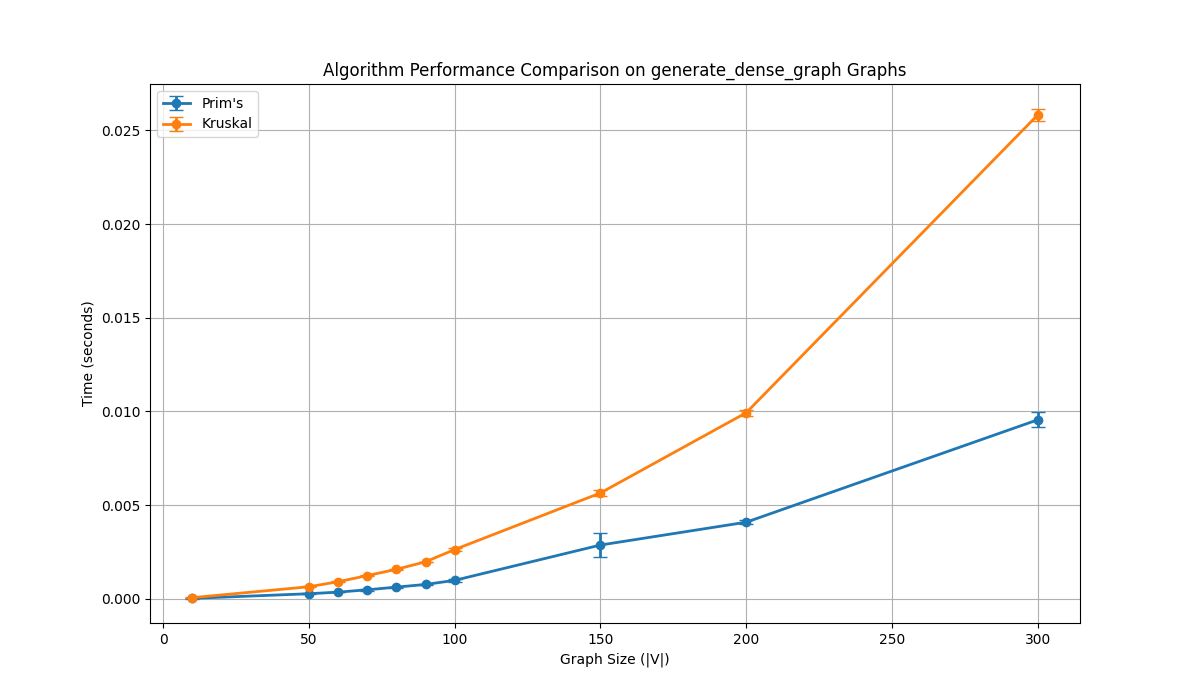
\includegraphics[width=.9\linewidth]{mst_dense.png}
\label{org4fa743f}
\end{center}

In dense graphs (approximately 80\% of maximum possible edges), we observe similar performance patterns to complete graphs, but with proportionally reduced execution times.

Based on the figure, Prim's algorithm maintains a substantial advantage over Kruskal's algorithm. For a dense graph with 300 vertices, Prim's algorithm takes approximately 0.01 seconds, while Kruskal's algorithm requires about 0.026 seconds - still more than twice as long.

This performance difference is consistent with what we observed in complete graphs and reinforces that Prim's algorithm is better suited for graphs with high edge density. The algorithm's approach of growing a single tree from a starting vertex efficiently handles densely connected graphs where there are many candidate edges to consider at each step.

The error bars remain small, indicating reliable and consistent measurements across test runs.
\subsection{Sparse Graph}
\label{sec:org274af69}
\begin{center}
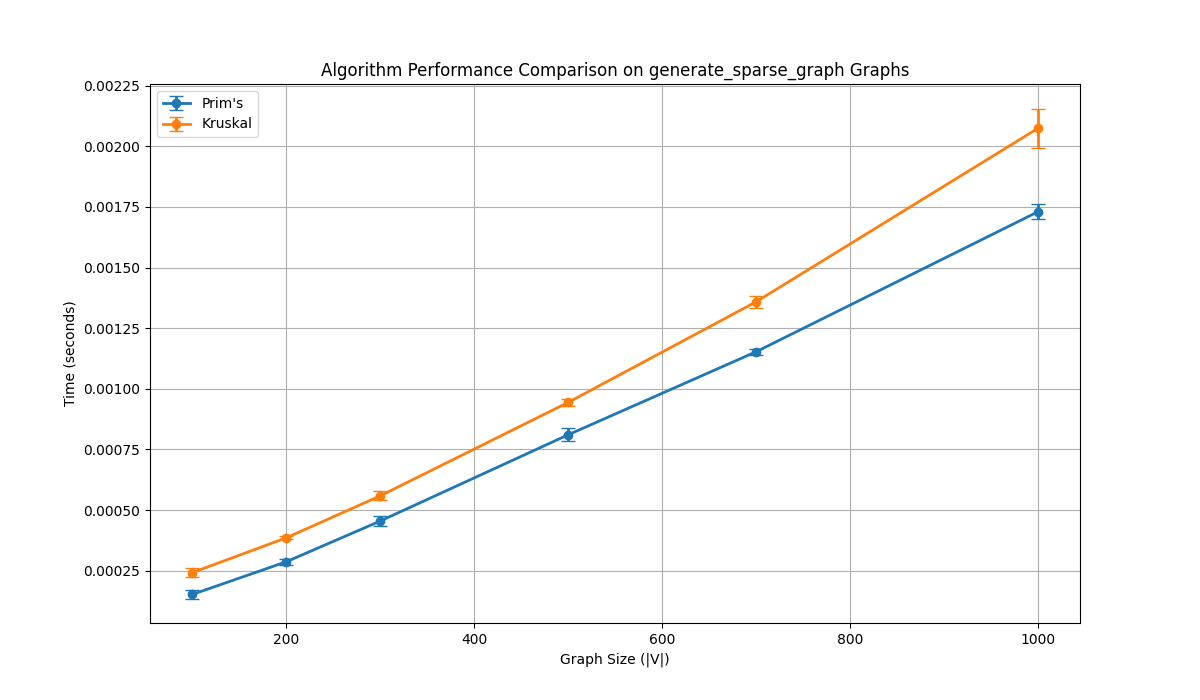
\includegraphics[width=.9\linewidth]{mst_sparse.png}
\label{org7dccec3}
\end{center}

For sparse graphs (with approximately 2|V| edges), the performance characteristics of both algorithms change significantly compared to dense graphs.

Based on the figure, both algorithms exhibit a nearly linear growth pattern with increasing graph size, which is consistent with their theoretical O(E log V) complexity when E is proportional to V. 

Notably, in sparse graphs, both algorithms perform comparably, with slightly better performance from Prim's algorithm. For a sparse graph with 1000 vertices, Prim's algorithm takes approximately 0.00175 seconds, while Kruskal's algorithm requires about 0.0021 seconds.

This relatively small difference (compared to the much larger gap seen in dense graphs) can be explained by Kruskal's algorithm needing to sort far fewer edges in sparse graphs. While Prim's algorithm still maintains an advantage, the performance gap is significantly reduced.

The standard deviation is slightly higher than in dense graphs but still indicates consistent measurements across test runs.
\subsection{Connected Graph}
\label{sec:org2c4a35e}
\begin{center}
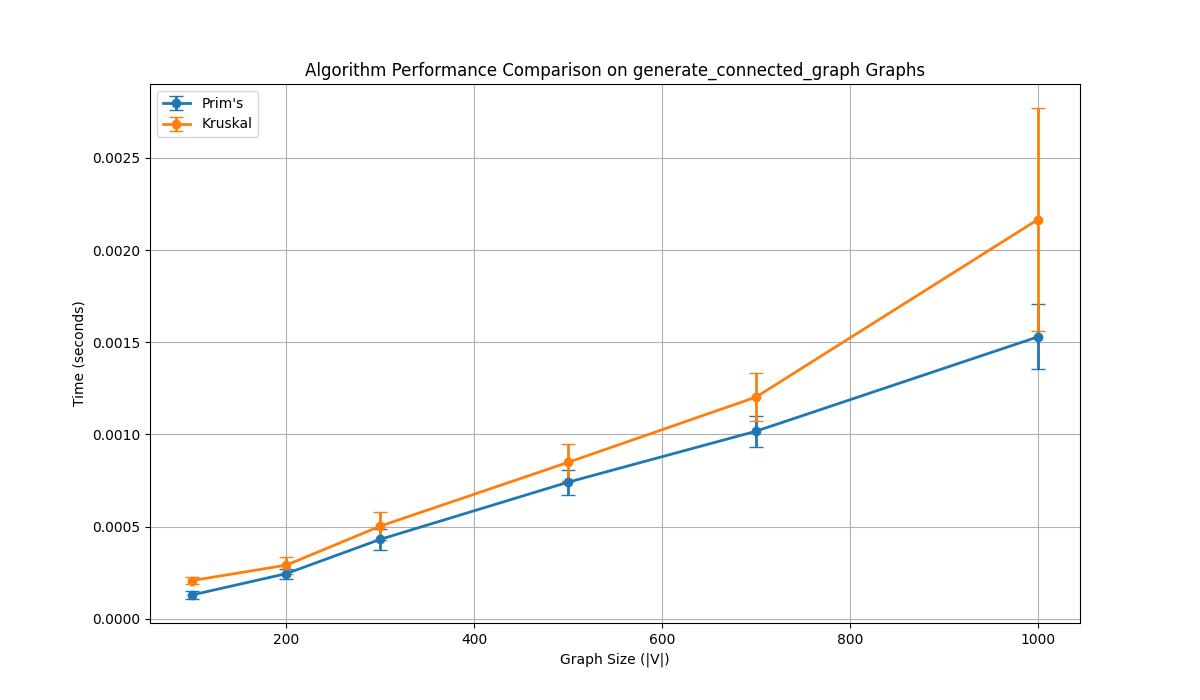
\includegraphics[width=.9\linewidth]{mst_connected.png}
\label{org1a55bc6}
\end{center}

Connected graphs show a linear growth pattern for both algorithms, similar to sparse graphs.

According to the figure, both Prim's and Kruskal's algorithms perform comparably, with Kruskal's algorithm showing slightly higher execution times. For a connected graph with 1000 vertices, Prim's algorithm takes approximately 0.0015 seconds, while Kruskal's requires around 0.0022 seconds.

This performance difference is consistent but not as pronounced as in dense or complete graphs. The connected graphs used in this test likely have moderate edge density, leading to balanced performance between the two algorithms.

The error bars increase with graph size but remain relatively small, indicating reliable measurements with some expected variability.
\subsection{Grid Graph}
\label{sec:orge463fee}
\begin{center}
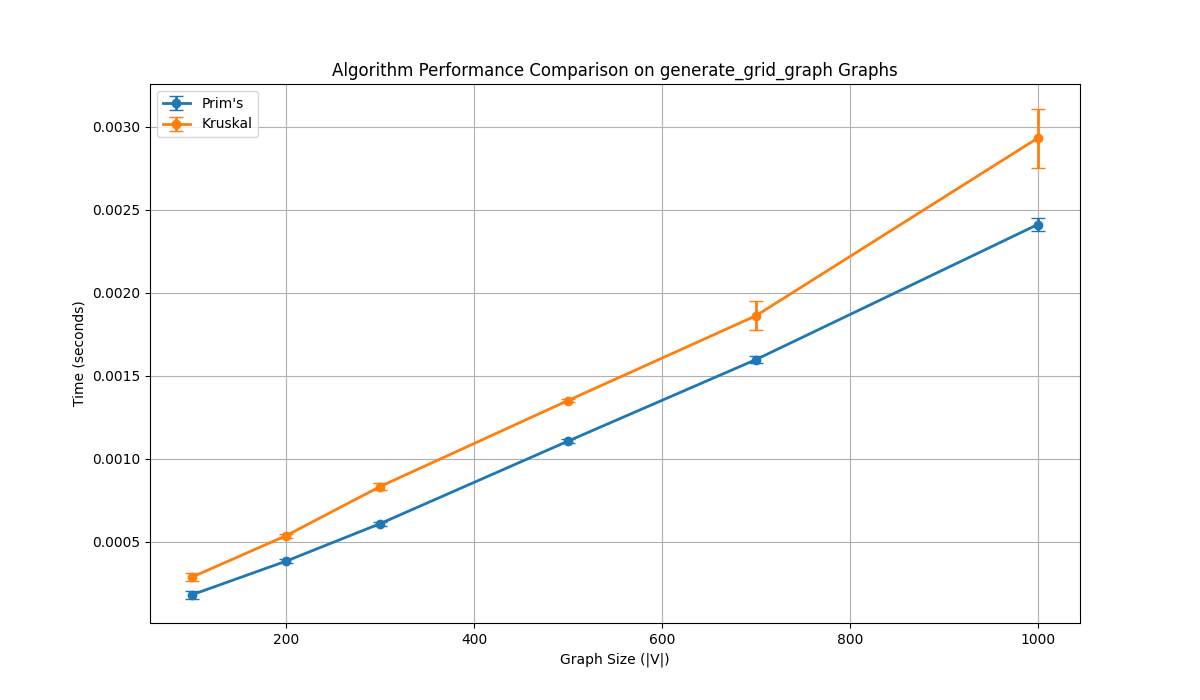
\includegraphics[width=.9\linewidth]{mst_grid.png}
\label{orgcad8889}
\end{center}

Grid graphs present an interesting case for MST algorithms due to their regular structure.

Based on the figure, both algorithms show linear growth with graph size, but Prim's algorithm consistently outperforms Kruskal's algorithm. For a grid graph with 1000 vertices, Prim's algorithm takes approximately 0.0024 seconds while Kruskal's requires around 0.0029 seconds.

The performance advantage of Prim's algorithm for grid graphs is noteworthy considering that grid graphs are relatively sparse (maximum 4 edges per vertex). This suggests that Prim's approach of growing a connected tree is particularly efficient for the structured nature of grid graphs, where edges have a predictable pattern of connectivity.

The standard deviation is small relative to the mean values, indicating consistent measurements across test runs.
\section{Conclusions}
\label{sec:org163100e}

This laboratory work demonstrates that the relative performance of Prim's and Kruskal's algorithms varies based on graph density and structure, despite having the same asymptotic complexity of O(E log V).

The empirical analysis reveals several key insights:

Prim's algorithm consistently outperforms Kruskal's algorithm in dense and complete graphs. For complete graphs with 300 vertices, Prim's algorithm is approximately three times faster than Kruskal's. This advantage stems from Prim's efficient approach of growing a single tree from a starting vertex, which avoids the costly sorting of all edges required by Kruskal's algorithm.

In sparse graphs, connected graphs, and grid structures, the performance difference between the two algorithms is less pronounced. Prim's algorithm still maintains an advantage in most cases, but the margin is smaller. This reduced gap is due to the smaller number of edges that Kruskal's algorithm needs to sort.

Both algorithms scale according to their theoretical complexity predictions, with execution time growing as O(E log V). The results confirm that the constant factors and actual performance characteristics vary significantly based on graph structure.

Implementation details matter significantly. Our implementation uses a binary heap for Prim's algorithm and a disjoint-set data structure for Kruskal's algorithm. Different data structures could potentially change the performance characteristics.

The consistency of results across repetitions (small standard deviations) indicates that both algorithms have stable performance characteristics, making them reliable choices for MST problems.

These findings highlight the importance of understanding both the theoretical complexity and practical performance characteristics when choosing between MST algorithms. While both algorithms are viable solutions for finding minimum spanning trees, Prim's algorithm appears to be the better choice in most scenarios tested, particularly for denser graphs.

For applications where graph density is known in advance, this analysis provides clear guidance on algorithm selection: use Prim's algorithm for dense graphs, and consider either algorithm for sparse or structured graphs with a slight preference for Prim's if performance is critical.
\end{document}
